\chapter{Estado del arte}\label{sec:eda}

\section{Simuladores de eventos discretos}

Un sistema es una colección de entidades que interactúan bajo ciertas reglas
para alcanzar un fin común. Decimos que un sistema es \textit{continuo} cuando
las variables que permiten describir su estado cambian de forma contínua con
respecto al tiempo (por ejemplo, altura y velocidad de un avión). En oposición,
los sistemas \textit{discretos} son aquellos en los que las variables de estado
cambian de forma instantánea en determinados momentos en el tiempo (por
ejemplo, cantidad de clientes en una estación de servicio).

A menudo es de interés estudiar un sistema para entender los parámetros que
gobiernan su funcionamiento, realizar mejoras o comprender de qué manera serán
impactados por ciertos cambios en sus entradas.

Para llevar a cabo un estudio de esta naturaleza, una primera opción es
experimentar con el sistema real. No obstante, esto no siempre es deseable
(podría implicar muchos gastos y disrupciones en el funcionamiento normal del
sistema) o siquiera posible (quizás el sistema aún no ha sido construido).
Entonces se puede recurrir a experimentar con un \textit{modelo} del sistema.

Un modelo puede ser \textit{físico} (modelo a escala) o \textit{matemático}.
Este último consiste en una serie de suposiciones sobre el funcionamiento del
sistema que se pueden formalizar en un conjunto de relaciones matemáticas y
lógicas entre las entidades que lo componen.

A veces un sistema es lo suficientemente sencillo como para que el modelo
matemático del mismo pueda ser resuelto analíticamente, mediante el uso de
herramientas tales como el cálculo diferencial, álgebra, teoría de
probabilidad. Sin embargo, cualquier modelo más o menos interesante de un
sistema no trivial suele ser muy complejo para ser tratado mediante estos
métodos. Aparece entonces la simulación como una forma de ganar comprensión
sobre el funcionamiento del sistema.

% TODO: confirmar la fuente de este diagrama

\begin{figure}[h]
\caption{Formas de estudiar un sistema \cite{law}}
\centering
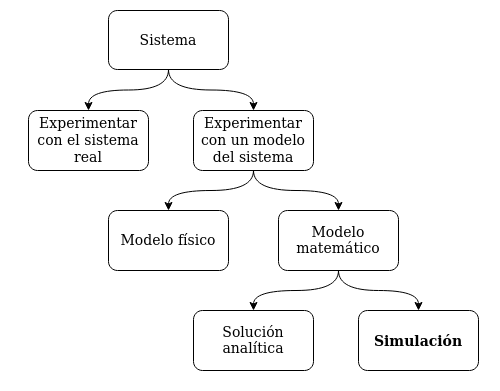
\includegraphics[width=8cm]{taxonomia}
\end{figure}

En una simulación, el modelo no es resuelto, sino que es \textit{ejercitado}
con el fin de recolectar información a partir de la cual se puedan realizar
estimaciones sobre los valores de los parámetros de interés.

La construcción de una simulación ofrece las siguientes ventajas:
\begin{itemize}
    \item Nuevas políticas, procedimientos de operación, reglas de decisión,
    flujos de información, procedimientos de organización, etc. pueden ser
    explorados sin perturbar la operación del sistema real.

    \item Nuevos diseños pueden ser probados sin asignar recursos a la
    adquisición de elementos físicos, antes de implementar cambios en el mundo
    real.

    \item Permite validar hipótesis y responder a preguntas de tipo ``¿qué
    pasaría si...?''.

    \item El diseño de la simulación permite ganar conocimiento sobre el
    sistema bajo investigación.

    \item Permite cambiar los valores de entrada para observar cambios en las
    salidas, lo cual facilita una mayor comprensión sobre cuáles son las
    variables más relevantes y cómo interactúan.

    \item Proporciona una herramienta de gran valor pedagógico.

    \item Permite verificar soluciones analíticas.

    \item El tiempo es artificial, y por lo tanto puede ser contraído (simular
    meses o años de funcionamiento de un sistema en algunos minutos), expandido
    (observar cambios que de otra forma serían demasiado rápidos) e incluso
    pausado y avanzado manualmente.

    \item El concepto básico de una simulación es fácil de interpretar, por lo
    tanto puede ser una herramienta útil a la hora de justificar decisiones a
    clientes, inversores, gestores, etc.

    \item Puede ser más confiable que un modelo matemático resuelto de forma
    analítica, porque necesita hacer menos simplificaciones.
\end{itemize}

En los modelos estáticos no es relevante el paso del tiempo. Un ejemplo de
simulación de este tipo lo ofrece el método Monte Carlo. En los modelos
dinámicos, en cambio, el tiempo es relevante ya que se estudia la evolución del
sistema a través de una línea temporal artificial.

La simulación de eventos discretos involucra el modelado de un sistema y su
evolución mediante una representación en la cual las variables de estado
cambian de forma instantánea en determinados puntos del tiempo. Estos puntos
del tiempo son aquellos en los que un evento ocurre, donde un evento está
definido como una ocurrencia instantánea que tiene la potencialidad de cambiar
el estado del sistema. Decimos que hay una potencialidad de cambiar el estado
del sistema porque un evento puede utilizarse de manera que no cambie el
sistema pero que cumpla otros fines. Por ejemplo, se puede programar un evento
que dará fin a la simulación en un tiempo particular.

Si bien en principio sería posible llevar a cabo una simulación de eventos
discretos a mano, registrando el estado del modelo ante cada nuevo evento, la
cantidad de información que habría que manipular para simular cualquier sistema
del mundo real hace que esta tarea sólo sea abordada mediante el uso de
software especializado.

Un simulador de eventos discretos es un programa destinado a soportar la
simulación de sistemas mediante modelos dinámicos y discretos. En dichos
programas es común encontrar los siguientes componentes:

\begin{itemize}
    \item Estado del sistema: colección de variables necesarias para describir
    el sistema en un punto particular del tiempo.

    \item Reloj de simulación: una variable especial para llevar cuenta del
    tiempo.

    \item Lista de eventos: una lista con los eventos futuros.

    \item Contadores: variables usadas para almacenar información estadística
    sobre el desempeño del sistema.

    \item Fuentes de variables aleatorias para las distribuciones más comunes.

    \item Herramientas de recolección y manipulación de datos, procesamiento
    estadístico y representación visual de los mismos.

    \item Interfaz gráfica que proporciona una representación visual del
    sistema (en dos o tres dimensiones), mostrando animaciones que ayudan al
    seguimiento de los cambios de estado.
\end{itemize}

Las fuentes consultadas en la confección de este capítulo fueron \cite{law},
\cite{banks}, \cite{shannon}.

\section{Simulador \omnetpp{}}

Objective Modular Network Testbed in C++ (\omnetpp{}) es un simulador de eventos
discretos modular y orientado a objetos, escrito en el lenguaje de propósito
general C++. Originado en 1997 por András Varga, es un software de código
abierto que puede ser utilizado libremente para usos no comerciales
(principalmente investigación y enseñanza). Existe una extensión de \omnetpp{}
para usos comerciales llamada OMNEST.

Principalmente orientado a la simulación de sistemas de comunicación,
multiprocesadores y otros sistemas distribuidos, \omnetpp{} es lo suficientemente
general como para resultar de utilidad en otros dominios (diseño de protocolos,
validación de arquitecturas de hardware, evaluación de desempeño de sistemas de
software, y en general, cualquier sistema donde el enfoque de eventos discretos
sea apropiado y pueda ser convenientemente mapeado a un conjunto de entidades
que intercambian mensajes).

Su diseño modular hace posible que ciertas piezas centrales de la simulación de
redes que no son parte del paquete principal (por ejemplo, librerías de
simulación de protocolos TCP) aparezcan espontáneamente desde una comunidad de
usuarios muy activa.

\omnetpp{} hace mucho énfasis en la facilidad de depuración y trazabilidad de
los elementos constituyentes del modelo, para lo cual es posible ejecutar las
simulaciones en un ambiente de interfaz gráfica que presenta animaciones para
los eventos (mensajes) y brinda facilidad de inspección de los módulos
intervinientes.

También es posible ejecutar simulaciones en un ambiente de consola (es decir,
sin interfaz gráfica), útil para la ejecución en lote de varios experimentos.

Ofrece soporte para simulaciones de gran escala preparadas para ser
paralelizadas en un cluster de computadoras.

Busca apoyarse en interfaces abiertas (archivos de texto plano, formatos
comunes) para posibilitar la interacción con otras herramientas.

\subsection{Introducción a \omnetpp{}}

En esta sección se describen en detalles los diferentes componentes de un
modelo de simulación de \omnetpp{} desde la perspectiva del usuario.

\paragraph{Modelos y estructura jerárquica}

En \omnetpp{}, un modelo consiste de módulos que se comunican mediante el paso de
mensajes. Los módulos simples se escriben en el lenguaje de programación C++,
utilizando clases de la librería de simulación. Estos módulos simples
constituyen el componente atómico (no se pueden subdividir) y activo (es donde
el usuario introduce la lógica del modelo) del modelo.

Estableciendo una estructura jerárquica sin límite de niveles, los módulos
simples pueden ser agrupados en módulos compuestos, lo cual permite dividir los
modelos complejos en partes más pequeñas, o agrupar varias partes en un único
módulo. Esta es una decisión de diseño que corre por cuenta del usuario. 

Los módulos se comunican mediante el paso de mensajes. Además de una marca de
tiempo, los mensajes pueden tener cualquier tipo de atributo. Los módulos
presentan compuertas de entrada y de salida que constituyen su interfaz.  Los
mensajes usualmente se destinan a compuertas, pero también es posible enviarlos
directamente a módulos específicos.

Los módulos pueden tomar parámetros, utilizados para pasar configuraciones y
definir la topología del sistema. Asimismo, las conexiones entre módulos pueden
tener atributos (demora de propagación, tasa de error, tasa de transferencia),
permitiendo definir conexiones como tipos (canales) para reutilizarlos.

Los parámetros pueden tomar valores específicos, declarados en archivos de
configuración, o pueden ser tomados de una fuente de valores aleatorios. 

\paragraph{El lenguaje NED}

NED es un lenguaje declarativo que fue creado específicamente para \omnetpp{},
en el cual el usuario define la estructura del modelo (módulos e
interconexiones).

Una definición de modelo puede constar de declaraciones de módulos simples,
módulos compuestos y definiciones de la red:

\begin{itemize}
    \item Los módulos simples describen su interfaz: compuertas y parámetros.

    \item Los módulos compuestos son definidos mediante la declaración de su
interfaz externa (compuertas y parámetros) así como la definición de sus
submódulos y sus interconexiones.

    \item La definición de una red típicamente declara al modelo como una
instancia de un módulo particular.
\end{itemize}

Las definiciones NED soportan la partición en diferentes archivos mediante el
mecanismo de inclusión.

\omnetpp{} incluye un editor gráfico que toma como partida los archivos NED. El
usuario puede hacer cambios tanto en la vista gráfica como directamente en el
texto del archivo, y cambiar de vista en cualquier momento.

NED es un lenguaje declarativo que contiene constructos parecidos a los
condicionales y los bucles de un lenguaje imperativo, lo que posibilita
parametrizar las topologías. Esto es una ventaja sobre otros simuladores donde
o bien no es posible parametrizar (sólo se pueden expresar topologías fijas) o
donde la especificación del modelo se mezcla con la lógica de la simulación,
haciendo imposible la edición gráfica.

El lenguaje NED es compatible con el formato XML, lo que posibilita la carga
dinámica de modelos que provengan de otras fuentes.

\paragraph{Programación de módulos simples}

Los módulos simples son los elementos activos del sistema y funcionan como
bloques constituyentes de los módulos complejos y, en última instancia, del
modelo de simulación.

El usuario implementa la funcionalidad de un módulo simple heredando de la
clase \verb!cSimpleModule!, que es parte de las librerías de simulación de
\omnetpp{} y puede optar por dos paradigmas de programación diferentes:

\begin{itemize}
    \item basado en corrutinas
    \item basado en el procesamiento de eventos
\end{itemize}

En el paradigma basado en corrutinas, el código del modelo corre en su propio
hilo, el cual recibe el control del kernel de simulación cada vez que el módulo
recibe un mensaje. Típicamente, este código nunca incluye un \verb!return!: sus
puntos de entrada son llamadas a \verb!receive! (esperar el siguiente mensaje)
y sus puntos de salida son llamadas a \verb!send! (enviar un mensaje)

En el paradigma basado en el procesamiento de eventos, el kernel de simulación
llama a una función específica del módulo (\verb!handleMessage!) con el mensaje
como argumento. Esta función debe ejecutar un \verb!return! al terminar de
procesar el mensaje, efectivamente devolviendo el control al kernel de
simulación.

Además de el código destinado al envío y recepción de mensajes, es posible
escribir código que se ejecuta durante la inicialización y finalización del
módulo (este último, sólo si la simulación terminó exitosamente).

Como parte de la simulación, un módulo puede cambiar sus entradas y salidas, o
crear dinámicamente nuevos módulos, lo cual hace posible modificar la topología
inicial de la red.

\paragraph{Separación del modelo y los experimentos}

Como se describió anteriormente, el comportamiento del modelo es capturado en
archivos C++ mientras que la topología es capturada en archivos NED.

En una simulación cualquiera, uno está generalmente interesado en conocer cómo
se comporta el modelo a partir de diferentes datos de entrada. Esta información
no pertenece ni a los archivos C++ ni a los archivos NED: la configuración de
los experimentos se coloca en otros archivos, con extensión \verb!ini!. En
ellos se puede especificar cuántas corridas de una simulación se desea
realizar, con qué valores para los parámetros, con qué distribuciones
aleatorias, cuánto tiempo puede durar como máximo la simulación, etc.

\paragraph{Entorno de desarrollo integrado}

La edición de los diferentes archivos que intervienen (archivos de C++,
archivos NED, archivos \texttt{ini}) puede realizarse cómodamente desde un Entorno de
Desarrollo Integrado (IDE, por sus siglas en inglés) que es parte de la
distribución oficial de \omnetpp{}. Las ventajas de programar desde este IDE son
múltiples:

\begin{itemize}
    \item Introspección de código, navegación a la definición de una variable,
navegación a la documentación.

    \item Asistencia para operaciones comunes de refactorización de código.

    \item Acceso rápido a funcionalidades comunes como compilación o ejecución.

    \item Resaltado de sintaxis de los diferentes lenguajes

    \item Depuración de código.

    \item Asistente para la generación de nuevos proyectos.

    \item Edición de archivos NED desde la vista gráfica.
\end{itemize}

A su vez, este entorno de desarrollo integrado ofrece la posibilidad de
visualizar gráficos de diversos tipos a partir de los datos generados durante
una simulación.

\paragraph{Ejecución de una simulación}

El código de los módulos simples se compila enlazando con las librerías de
simulación de \omnetpp{} creando un binario que constituye el ejecutable de la
simulación. Cambios posteriores a los archivos NED (cambios en la topología y
en los parámetros) o en los archivos \verb!ini! (cantidad y duración de las
simulaciones, distribuciones de las variables aleatorias, valores de los
parámetros) no requieren nuevos pasos de compilación.

El binario de la simulación puede ejecutarse de forma que la misma se
corra en un entorno gráfico apto para la visualización y depuración del modelo,
o sin este entorno gráfico (más apropiado para correr muchas simulaciones en
lote).

\subsection{Ecosistema y casos de uso}

Desde sus comienzos, cerca del año 2000, \omnetpp{} ha tenido una amplia
recepción en entornos de investigación, educativos, así como también en la
industria.  Diversos proyectos independientes han aportado nuevas librerías
reutilizables y modelos de dominios específicos, algunos de los cuales se
listan a continuación\footnote{Para una lista completa, visitar
\url{https://omnetpp.org/download/models-and-tools}}.

\begin{itemize}
    \item INET Framework (\url{https://inet.omnetpp.org}) provee soporte para
    simulaciones de redes de comunicación que utilizan los protocolos de
    Internet (TCP, UDP, IPv4, IPv6, OSPF, BGP, etc.), así como protocolos
    cableados e inalámbricos de la capa de enlace (Ethernet, PPP, IEEE 802.11,
    etc.) y soporte para redes móviles, protocolos MANET (Mobile Ad Hoc
    Networks), DiffServ, etc. Muchos otros proyectos toman INET como base y la
    extienden en direcciones específicas, como redes de vehículos, overlay,
    P2P, LTE.

    \item Simu5G (\url{http://simu5g.org/}) producto de un proyecto de
    investigación conjunta entre Intel Corporation y el Computer Networking
    Group de la Universidad de Pisa, Italia, provee soporte para redes 5G
    NewRado \cite{Simu5G}.

    \item SimulLTE (\url{https://simulte.com/}) provee librerías para la
    simulación de redes LTE y LTA \cite{SimuLTE}.

    \item Veins (\url{https://veins.car2x.org}) es un framework de simulación
    de código abierto de IVC (Inter-Vehicular Communication) que utiliza
    \omnetpp{} para la simulación de redes así como SUMO, un simulador de
    tráfico vehicular, usando cosimulación \cite{Veins}.

    \item CoRE4INET (\url{https://core-researchgroup.de/projects/simulation.html})\linebreak
    es una extensión a la herramienta INET para simulaciones basadas en eventos
    de real-time Ethernet dentro del simulador \omnetpp{}.
\end{itemize}

Desde el año 2008 en forma continuada, la comunidad de \omnetpp{} se reúne
anualmente en un evento en el que se comparten experiencias, casos de usos y se
realizan ``hackatones'', maratones de programación en los que se busca atacar
un problema concreto de forma creativa en pocas horas. Algunos de los temas
presentados:

\begin{itemize}
    \item Development and Testing of Automotive Ethernet-Networks together in
    one Tool - \omnetpp{} (Patrick Wunner, Stefan May, Kristian Trenkel, and
    Sebastian Dengler)

    \item Implementation of an Adaptive Energy-efficient MAC Protocol in
    \omnetpp{} / MiXiM (Van Thiep Nguyen, Matthieu Gautier, and Olivier Berder)

    \item Attack of the Ants: Studying Ant Routing Algorithms in Simulation and
    Wireless Testbeds (Michael Frey and Mesut Günes)

    \item Modeling Quantum Optical Components, Pulses and Fiber Channels Using\linebreak
    \omnetpp{} (Ryan D. L. Engle, Douglas D. Hodson, Michael R. Grimaila, Logan
    O.  Mailloux, Colin V. McLaughlin and Gerald Baumgartner)

    \item High Frequency Radio Network Simulation Using \omnetpp{} (Jeffery
    Weston and Eric Koski)

    \item Stacked-VLAN-Based Modeling of Hybrid ISP Traffic Control Schemes and
    Service Plans Exploiting Excess Bandwidth in Shared Access Networks (Kyeong
    Soo Kim)

    \item DoS Protection through Credit Based Metering - Simulation Based
    Evaluation for Time-Sensitive Networking in Cars (Philipp Meyer, Timo
    Häckel, Franz Korf and Thomas Schmidt).
\end{itemize}

Para una lista completa se recomienda visitar la página oficial de los archivos
de la conferencia en \url{https://summit.omnetpp.org/archive/}.

Las fuentes consultadas en la confección de este capítulo fueron \cite{varga1},
\cite{varga2}, \cite{opp_manual}.

\section{Otras herramientas similares}

Esta sección presenta brevemente los principales proyectos que cumplen el rol
de simulador de eventos discretos, sus características y sus diferencias con
\omnetpp{}. En particular, se toma el caso de SimPy que es, hasta donde alcanza
nuestro conocimiento, el único programa de este tipo basado en el lenguaje
Python.

\subsection{ns3}

Herramienta orientada a la simulación de redes de comunicación, dirigido
principalmente al uso académico y educativo. Es un proyecto de
código abierto, gratuito, liberado bajo la licencia GNU GPLv2 mantenido por su
comunidad. Está basado en C++ y parte de la API de simulación cuenta con
``bindings'' (enlaces) para Python que son generados automáticamente (hasta
donde este proceso es automatizable) y cuya completitud y correctitud no es el
principal objetivo del proyecto \cite{ns3page} \cite{ns3pagepython}.

A diferencia de \omnetpp{}, la simulación y la visualización (depuración,
trazabilidad) son temas separados. Por defecto, no presenta interfaz gráfica
para mostrar animaciones de los modelos. Las trazas generadas durante una
simulación pueden procesarse en otro software denominado NetAsim que permite la
visualización, o incluso en otros programas no relacionados, como WireShark.
Existe también una extensión (PyViz) que permite realizar una visualización
interactiva (es decir, durante la simulación) pensada con propósitos de
depuración.

A pesar de su filosofía de modularización, esta herramienta no separa los
múltiples aspectos de una simulación (lógica, configuración, topología) en
diferentes archivos, si no que todo esto se realiza directamente mediante el
código C++. Por esta razón, el usuario tiene que proveer más código C++ que en
una simulación típica de \omnetpp{}, ya que el programa incluye desde el
tratamiento de los argumentos del programa (si los hubiere), la declaración y
configuración de los nodos, los canales, las aplicaciones, el nivel de logging,
etc, hasta la misma inicialización y finalización de la simulación.

Es una herramienta que supone que el usuario está muy familiarizado con el
entorno de línea de comandos y puede configurar y compilar sus fuentes con
facilidad para producir el binario adaptado a sus necesidades.

\subsection{NetSim}

NetSim parece ser un nombre bastante común para este tipo de software. En
particular, aquí hablamos de la herramienta producida por la compañía india
Tetcos (\url{https://www.tetcos.com/}). NetSim v1 apareció en 2005 y se
encuentra actualmente en la versión 13 (mayo 2021).

Esta herramienta, escrita en lenguaje C, corre sobre plataformas Windows y se
distribuye bajo diferentes licencias comerciales. Existe incluso una licencia
especial para usos académicos y educativos, que también es paga.

Está orientada a la simulación de redes de comunicación, para lo cual provee
una extensa librería con los protocolos y elementos necesarios (de acuerdo al
tipo de licencia obtenida).

El principal caso de uso es el de establecer un escenario de simulación
ubicando componentes (nodos, aplicaciones, enlaces) en una grilla espacial, y
caracterizando los canales de comunicación, para luego correr la simulación y
recoger métricas que permitan sacar conclusiones.

El usuario sólo puede implementar sus propios algoritmos o recolectores de
datos editando el código fuente de NetSim y volviendo a compilar.

\subsection{SimPy}

Se trata de una librería de código abierto para escribir simulaciones de
eventos discretos en lenguaje Python, distribuida bajo una licencia MIT que
posibilita su uso libre \cite{sympy}.

La simulación se estructura alrededor del concepto de \textit{proceso}, que
constituye el elemento activo de la simulación (un cliente, un coche, un nodo
de una red), haciendo uso de generadores.

En Python, un generador es un tipo especial de función que incluye la palabra
reservada \verb!yield!. Al ejecutar la instrucción \verb!yield!, la función es
pausada y el control retorna al código que la llamó. Posteriormente, la
ejecución de la corrutina se puede reanudar, desde el mismo punto donde cedió
el control.

Esta característica del lenguaje Python ofrece un recurso que SimPy utiliza
para estructurar la simulación, en un modelo de corrutinas (funciones que ceden
el control voluntariamente en lo que se denomina concurrencia cooperativa). Los
generadores crean eventos y ceden el control al orquestador de la simulación
cuando ejecutan un \verb!yield!. Cuando el evento \textit{ocurre} (llega su
momento en el tiempo de la simulación) el proceso continúa.

Simpy incluye también funcionalidad para modelar el uso de recursos
compartidos y la interacción de procesos.

Es importante notar que SimPy es simplemente una librería que implementa el
código básico para estructurar una simulación, pero no provee muchas de las
funcionalidades que las otras herramientas tienen incorporadas (interfaz
gráfica, animación, recolección de datos, configuración de experimentos,
visualización de resultados, etc.).

\section{C++ vs. Python}

Analizando herramientas de simulación de eventos discretos, lo más común es
encontrar que se ha utilizado un lenguaje de bajo nivel como C o C++, siendo
SimPy, hecho en Python, un caso excepcional. En esta sección se hace una breve
comparación entre C++ y Python, para entender qué se gana y qué se pierde al
utilizar cada lenguaje. Esto nos permitirá fundamentar mejor por qué este
proyecto toma la iniciativa de permitir la utilización de la herramienta
\omnetpp{} (escrita en C++) desde código escrito enteramente en Python.

\subsection{Generalidades}

Originado por Bjarne Stroustrup en 1979 como una extensión del lenguaje C que
añadía soporte para programación orientada a objetos, C++ fue concebido para la
programación de sistemas operativos y sistemas embebidos, así como para
software con recursos escasos, con metas tales como performance y eficiencia.
Ha sido utilizado en muchos otros contextos \cite{stroustrup}, como ser
aplicaciones de escritorio, videojuegos, servidores, y también en aplicaciones
de alta criticidad (enlaces telefónicos o sondas espaciales).

Se trata de un lenguaje compilado, por lo que se puede utilizar en cualquier
plataforma para la cual exista un compilador de C++.

En el año 1998, el lenguaje fue estandarizado por la International
Standarization Organization (ISO). A dicho estándar siguieron ampliaciones y
modificaciones en los años 2003, 2011, 2014, 2017, siendo el último estándar
publicado en 2020 en lo que se denomina informalmente C++20.

Python fue originado a finales de la década de 1980 por Guido Van Rossum, y
conoció su primera edición oficial en 1991. La versión más reciente del
lenguaje, al momento de escribir este documento, es la 3.10, liberada en
octubre de 2021. Desde sus inicios, el lenguaje ha puesto énfasis en producir
un lenguaje fácil de escribir y de leer, poniendo el acento en que el tiempo de
las personas es más valioso que el tiempo del CPU.

El desarrollo y crecimiento del lenguaje es guiado por una organización sin
fines de lucro llamada \href{https://www.python.org/psf/}{Python Software
Foundation}.

\subsection{Sintaxis}

C++ hereda su sintaxis del lenguaje C, terminando cada sentencia con punto y
coma y delimitando bloques por medio de corchetes. 

En general, Python tiene una sintaxis más sencilla, con menos palabras clave y
utiliza sangrías para definir bloques de código. Leer un programa en Python
muchas veces se puede asemejar a leer un texto en inglés.

\subsection{Forma de uso}

C++ es un lenguaje compilado. El código fuente es finalmente convertido a un
formato binario que puede ser ejecutado instrucción por instrucción por el
procesador de la computadora. Un paso intermedio realizado por una herramienta
conocida como ``preprocesador'' puede además realizar cambios en el conjunto de
caracteres escrito directamente por el programador, insertando otros archivos
(directiva \verb!#include!), incluyendo o excluyendo ciertos bloques (directiva
\verb!#ifdef!) o también expandiendo lo que comúnmente se conoce como ``macros''.
Esto agrega un nivel de dificultad más a la sintaxis de C++, ya que lo que el
programador escribe, no suele ser exactamente igual a lo que el compilador
recibe para convertir a binario.

Python no es un lenguaje compilado, como C++ o C, si no que es un lenguaje
interpretado: el código fuente no es convertido directamente a código máquina
para su ejecución en un procesador. El código escrito en Python debe ser
proporcionado a un programa especial que se conoce como ``intérprete''. Tras
una primera etapa de preprocesado (parseo, elaboración del AST, generación de
bytecode propio de Python), el intérprete se encarga de llevar adelante la
ejecución instrucción por instrucción. Este intérprete es en sí mismo un
programa que se llama comúnmente ``Python'' (o también Python3, Python35,
etc., dependiendo de la versión).

No existe un único intérprete de Python. El más popular y difundido, conocido
como ``cPython'', es el intérprete de referencia de Guido Van Rossum (creador
del lenguaje) escrito en C. Puede considerarse la implementación oficial: se lo
referencia como ``Python'' y se usa el término ``cPython'' (como en este
párrafo) cuando se busca distinguirlo de otras implementaciones \cite{pythonimpl}.

Notar que el término ``Python'' tiene (al menos) dos significados:

\begin{itemize}
    \item Es un lenguaje de programación definido mediante ciertas reglas
    sintácticas que delimitan las cadenas de caracteres que constituyen un
    programa válido y las separan de aquellas que, contrariamente, no son
    programas válidos (ver \url{https://docs.python.org/3/reference/grammar.html}).

    \item Es un binario que sirve de intérprete (ejecutor) de ciertos programas
    escritos usando tales reglas sintácticas.
\end{itemize}

A lo largo de este trabajo, cuando hablamos de ``Python'' nos referimos al
lenguaje. Para referirnos al binario que ejecuta archivos fuente en este
lenguaje, hablamos del ``intérprete'' o ``intérprete de Python''. Más
específicamente, nos referimos a la implementación oficial en C (cPython). 

\subsection{Distancia al hardware}

El factor que hace que un lenguaje sea considerado de alto o bajo nivel es su
distancia a los detalles físicos de la computadora que ejecuta el código.
En el nivel más bajo posible, podríamos intentar escribir un programa
cuidadosamente disponiendo ceros y unos de forma de componer un archivo binario
que llegara a ser ejecutable por el procesador. Un poco por encima de este
nivel, podríamos utilizar lenguaje assembly. Si bien aquí no se utilizan ceros
y unos directamente, sí se manipulan los registros del microprocesador, se
direcciona la memoria manualmente, se opera al nivel de bytes.

En general, en lenguajes de tan bajo nivel, se gana un control extremo sobre el
uso del hardware, pero se invierte un tiempo enorme en realizar tareas
triviales, y se hace en extremo difícil evitar errores.

Si bien C++ presenta muchas características de lenguaje de alto nivel, en
general no hay una gran abstracción sobre los detalles de una computadora. Por
el contrario, el lenguaje brinda herramientas para aprovechar esos detalles.
Como ejemplo, pensemos que quien programa tiene a su disposición diversos tipos
de datos para representar un entero (\verb!char!, \verb!int!, \verb!short int!,
\verb!long int!, \verb!long long int!, en sus versiones \verb!signed! o
\verb!unsigned!) lo cual permite elegir el más apropiado para cada aplicación
(según el rango de valores que se necesite representar, y la cantidad de
memoria que se pueda invertir en ello), pero también agrega un nivel de
dificultad extra para quien no domina los detalles, o simplemente no necesita
concentrarse en ellos. Python es considerado un lenguaje de alto nivel. No
busca exponer los detalles internos de la máquina
virtual ni de la máquina física subyacente. Esto, por supuesto, puede venir con
una penalidad en la performance y una ganancia en la usabilidad del lenguaje.

\subsection{Paradigmas soportados}

C++ es un lenguaje imperativo que puede utilizarse principalmente para escribir
programas de paradigma procedimental u orientado a objetos. Asimismo, una
característica del lenguaje que son los llamados templates o ``plantillas''
habilita a formas de programación genérica (código genérico cuya información de
tipo será definida en tiempo de compilación).

Python también es un lenguaje imperativo y soporta fuertemente los paradigmas
procedimental y orientado a objetos. Si bien no es un lenguaje funcional,
incluye características que permiten la adopción de un estilo de programación
funcional. Soporta también la programación orientada a aspectos y
metaprogramación.

\subsection{Sistema de tipos}

C++ emplea un sistema de tipos estático (toda variable tiene un tipo),
explícito (el tipo de la variable debe ser declarado, es parte del código
fuente). Como el tipo de cada variable se conoce en tiempo de compilación,
muchos errores de tipado son detectados y prevenidos por el compilador.

Python, en cambio, emplea un sistema de tipos dinámico, implícito (son los
valores de un programa -y no las variables- los que tienen tipo determinado,
pero estos tipos no son expresados como parte del programa). En general, esto
conduce a programas más fáciles de escribir y de leer, aunque no permite
detectar errores de tipos si no hasta que el código es ejecutado. Esto último,
sin embargo, no es visto como un problema en Python, por el contrario, se dice
que Python utiliza duck typing \cite{duck} (tipado del ``pato''), explicándolo
con la frase ``si camina como un pato y hace el sonido de un pato, entonces es
un pato''. En la práctica, esto quiere decir que Python favorece el paradigma
en el cual un objeto sirve en cualquier circunstancia donde pueda hacer lo que
se espera de él, independientemente de si tiene un tipo u otro. No se chequean
los tipos de los objetos (de hecho, herramientas del lenguaje que permiten
hacerlo como la función ``isinstance'', generan fuertes opiniones en contra de
su uso \cite{isinstance}) si no que se espera que un objeto pueda proveer el
comportamiento necesario (interfaz).

\subsection{Ecosistema}

C++, además del núcleo del lenguaje, provee la STL (Standard Template Library),
un conjunto de plantillas de clases que implementa muchos de los tipos de datos
más populares (listas, vectores, colas, stacks), así como algunos algoritmos. 

Python es considerado un lenguaje con ``baterías incluidas'' por la vastedad de
funcionalidad que se encuentra en su librería estándar. En ella encontramos
módulos para realizar operaciones comunes (manejo de fechas, establecer
comunicaciones http, compresión de archivos, envío de email, operaciones
comunes con texto y cadenas de caracteres, manejo de matrices, etc.) de forma
simple y sin escribir código especial.

Otros módulos que no son parte de la distribución oficial del lenguaje pueden
ser distribuidos e instalados mediante el uso de herramientas tales como
\verb!pip!, \verb!pipenv!, \verb!poetry! (manejadores de paquetes) a través de
repositorios de paquetes, siendo pypi.org el servidor oficial. Algunos paquetes
dentro de esta categoría han llegado a estandarizarse como las librerías por
defecto para realizar ciertas funciones:

\begin{itemize}
    \item visualización de gráficos: maptlotlib, pyplt
    \item procesamiento numérico: NumPy
    \item ciencia de datos: Pandas, SciKit-learn, PyTorch, TensorFlow, Keras
\end{itemize}

\subsection{Manejo de memoria}

En C++, las variables pueden ser alojadas dos tipos de
almacenamiento\footnote{Omitimos las variables en memoria estática, aquellas
que se declaran e inicializan en tiempo de compilación, por no ser relevantes
para esta discusión}:

\begin{itemize}
    \item Memoria automática (stack)
    \item Memoria manual (heap)
\end{itemize}

Las variables locales de cada función (especialmente cuando son valores que
caben en pocos bytes, como algunos enteros, caracteres, etc.) son almacenadas
en la pila o stack, y liberadas cuando la función hace \verb!return! (cuando el
activation record se remueve del stack). Esta memoria es manejada por el
compilador y el programador no necesita preocuparse por su manejo explícito.

Muchas veces, sin embargo, el programador debe recurrir a crear variables en el
heap (ya sea porque necesita alojar muchos objetos, o se trata de objetos
``grandes'', de varios bytes, que no caben en el stack). Este ``heap''
constituye una fuente de memoria que debe ser primeramente pedida al sistema
operativo y luego, cuando ya no es utilizada, debe ser devuelta. Fallar en
manejar correctamente este proceso implicaría la terminación inmediata del
programa (si trata de acceder a memoria no pedida) o la pérdida de recursos que
forman parte del ordenador pero que ya no pueden ser utilizados por ningún otro
proceso (al menos, hasta que termine la ejecución del programa). El programador
tiene que ser muy cuidadoso en este aspecto y suele ser uno de los elementos
más difíciles de la programación en C++.

En Python, el proceso de pedir, utilizar y devolver memoria es manejado
enteramente por un subsistema del intérprete o Python Runtime Environment. Al
momento de introducir variables o crear objetos, el programador puede confiar
que la memoria necesaria será pedida al sistema operativo, y esta será devuelta
a su momento. Todo es manejado automáticamente. Un subproceso informalmente
conocido como Garbage Collector (recolector de basura) se encarga de gestionar
qué porciones de memoria ya no están siendo referenciadas por ninguna variable
del programa y pueden, por lo tanto, ser recicladas o sencillamente devueltas
al sistema operativo.

En términos de practicidad, es claro que es más fácil programar en Python,
donde uno no necesita ni siquiera pensar en qué tipo de memoria están los
objetos, en pedir o devolver memoria, en pensar cuántos bytes ocupan, cómo
están alineados los objetos en relación a las direcciones de memoria, chequear
que la memoria está correctamente utilizada, etc. Todo esto está resuelto por
el intérprete. Pero, a su vez, tiene costos:

\begin{itemize}
    \item El algoritmo del Garbage Collector necesita tiempo para correr, y
    este tiempo es en detrimento de la ejecución de nuestra aplicación.

    \item El diseño de la gestión de la memoria busca minimizar el número de
    llamadas al sistema operativo y suele pedir recursos en bloques grandes,
    para gestión interna, conduciendo a aplicaciones que generalmente reservan
    más memoria de la estrictamente necesaria.
\end{itemize}

Otra razón por lo que los programas hechos en Python suelen usar más memoria
que programas equivalentes hechos en C++ es que en Python, todo es un objeto,
incluso valores de tipos básicos como puede ser un entero, internamente son
representados mediante objeto Python, lo cual ocupa mucho más que 4 bytes.

\subsection{C++ y Python como lenguajes de enseñanza}

Numerosos estudios comparativos entre Python y C++
\cite{zehra}\cite{Abdulkareem} muestran que el primero es menos eficiente que
el segundo (en términos de tiempo y espacio), en general por varios órdenes de
magnitud. Sin embargo, se señala que los programas hechos en Python son más
fáciles de entender y modificar. En general, las mismas características de C++
que lo hacen un lenguaje poderoso para administrar los recursos disponibles,
son aquellas que lo convierten en un lenguaje más difícil, propenso a errores
en manos no expertas. Se ha señalado que Python es un lenguaje más amigable
para novatos y más apropiado para la enseñanza de conceptos en ciencias de la
computación \cite{fraire}.
